\documentclass[main.tex]{subfiles}
\begin{document}
\section{The Data Sets}
The data presented in this chapter was collected during one hour of parallel measurements at the analog and the digital setup. The applied thresholds are shown in table \ref{tab:settings}. The YAP threshold was set at 9.8\si{\milli\volt} during acquisition, but having such a low threshold was found to decrease the signal to noise ratio in the time of flight spectrum, so a higher threshold of 24.4\si{\milli\volt} was applied.
\begin{table}[bh]
\begin{tabular}{|l|l|l|l|l|}
\hline
Setup   & YAP threshold(mV) & NE213 threshold(mV) & NE213 events ($\text{10}^\text{6}$) & Livetime \\ \hline
Analog  & 25.0              & 94.6                & 4.3      & 44\%             \\ \hline
Digital & 9.8/24.4	        & 48.8                & 2.2      & -             \\ \hline
\end{tabular}
\caption{Threshold values and number of NE213 events.}
\label{tab:settings}
\end{table}
\section{The Analog Setup}
\subsection{Pulse Shape Discrimination}
Neutrons and gamma rays were discriminated through the pulse shape parameter: 
\begin{equation}
PS=1-\frac{QDC_{sg}}{QDC_{lg}}
\end{equation}
Where QDC$_\text{lg}$ is the QDC value of the pulse integral over 500 ns and QDC$_\text{sg}$ is the value of the 60 ns integral. The baseline offset will constitute a larger fraction of deposited charge for smaller pulses than for larger pulses, so by adding a constant term to either the longgate or shortgate integration it is possible to change way PS varies as a function of energy. a constant 120 QDC channels was added to the shortgate QDC values, in order to linearize the pulse shape as a function of deposited energy. No constant was added to the longgate QDC values. 

Furthermore, events below 0.8 MeV are mostly the result of the pedestal injection, and consequently they are not of interest for pulse shape discrimination and have been removed. As can be seen from figure \ref{fig:qdc_a} there is some overlap between the injected YAP trigger distribution and the actual PuBe energy spectrum. This will be addressed when we look at the time of flight.

PS is shown as a function of deposited energy in figure \ref{fig:psd_a}. The upper band is made up of pulses for which the tail contained a large fraction of the total charge. This is the neutron band. Conversely The lower band is made up of gamma rays for which most of the energy is carried in the body of the pulse. That this is indeed true will be confirmed by the time of flight information.

\begin{figure}[ht]
    \centering
        \includegraphics{AnalogResults/psd.pdf}
        \caption{Heatmap of the fraction of total integrated charge as a function of energy. The dashed white line indicates the discrimination cut (tail/total = 0.259).}
        \label{fig:psd_a}
\end{figure}
In the analog setup a threshold of 94.6\si{\milli\volt} is applied. Since neutrons have a larger fraction of charge in the tail a 100 mV amplitude neutron signal can be expected to deposit more energy in the detector than a gamma ray pulse of equal amplitude. This gives rise to the curved energy threshold we see in the figure. It is also notable that the neutron band seems to be one single distribution, whereas the gamma band has two clear peaks. This is because the neutrons are produced with a more continuous distribution of energies whereas the gamma rays are produced with specific energies in the deexcitation of nuclei.

The linearization made it possible to draw a straight line through the spectrum, which separates neutrons from gammas. The procedure by which this cut was determined will be presented in parallel for the digital and the analog setup in chapter \ref{sec:results}. For now we just note that PS=0.259, shown as a dashed line in figure \ref{fig:psd_a}, was found to provide the best separation. Seeing how the neutron and gamma distributions seem to overlap at low energies this cut will likely cause some misclassification. Studying the time of flight can help us to get an idea of the extent of this misclassification.


\subsection{Time of Flight spectrum}
By correlating signals in the NE213 detector with those in the YAP we can tag neutrons and gammas in order to construct a time of flight spectrum. For practical reasons NE213 signals are used as start signals for the TDC while the gamma signals are delayed and used as stop signals. Thus the raw time of flight spectrum will contain a neutron peak to the left of a gamma peak. In figure \ref{fig:tof_a} this has been accounted for by switching the sign, converting from TDC channels to nanoseconds using the time calibration factor found in chapter \ref{sec:timecal}, and shifting the gamma peak to time t = 1.055 m/c (the approximate time it takes light to reach the NE213 detector). The energies of particles in the neutron peak is shown in the insert in the figure.

\begin{figure}[ht]
    \centering
        \includegraphics{AnalogResults/tof.pdf}
        \caption{The time calibrated time of flight spectrum. The x-axis denotes the time of flight from source to NE213 detector. The neutron and gamma peaks have been indicated with arrows and the upper right insert shows the energy distribution of events located in the neutron peak}
    \label{fig:tof_a}
\end{figure}

Since all the gamma rays travel at the speed of light one might expect a much narrower gamma peak. The are a number of reasons why this is not the case. First of all the gamma source and the detectors all have some size, so there are multiple paths light can take from source to detector. Secondly interactions are stochastic, so each gamma ray will travel some distance into a detector before interacting, which is particularly relevant for the much larger NE213 detector. The distance travelled through cables and the various electronic components, will also cause some attenuation, which may lead to differences in risetime of low and high amplitude pulses. This will in turn make the constant fraction discriminator less effective causing some loss in the time resolution. Furthermore, the final  digitization by the TDCs may cause some loss of resolution.

Since the distance from source to detector is known we can convert the neutron time of flight into Energy. The insert in figure \ref{fig:tof_a} shows the energy of particles located in the neutron peak, with higher flight times mapping to lower energies. The interval used is highlighted by the red dotted lines.


The time of flight information can offer insight into the energy cut made to separate out the pedestal events as well as the pulse shape discrimination cut. Figure \ref{fig:tof_ps_a} shows pulse shape as a function of time of flight, with neutron and gamma distributions highlighted. It is clear that it is not possible to make a discrimination cut on the pulse shape parameter without significant misclassification. 

Often the start and stop signal will be due to random coincidences. On small timescales of a few hundred nanoseconds these events are expected to form a flat background in the time of flight spectrum, as seen in figure \ref{fig:tof_a} beyond 60 ns. Since the events still represent either neutrons or gamma rays one would expect them to be separated into two bands in figure \ref{fig:tof_ps_a}. One above and one below the cut. However the distributions are not far enough from one another for this to be visible.

Another interesting feature is that there is large amount of gammas at higher PS values. This is because not all the unwanted YAP trigger induced events were removed by the cut at 0.8 $\text{MeV}_\text{ee}$ and as these events use the same signal as start and stop, they will appear to be simultaneous. The reason why they appear to have such a high fraction of tail/total lies in the gate lengths. Since the charge integrals of these events are just integrals of what randomly happened to be in the detector at the time a YAP trigger occured, and since the longgate window is more than eight time as long as the shortgate window it is more likely that there is something to integrate in the tail part of the window.
\begin{figure}[ht]
    \centering
        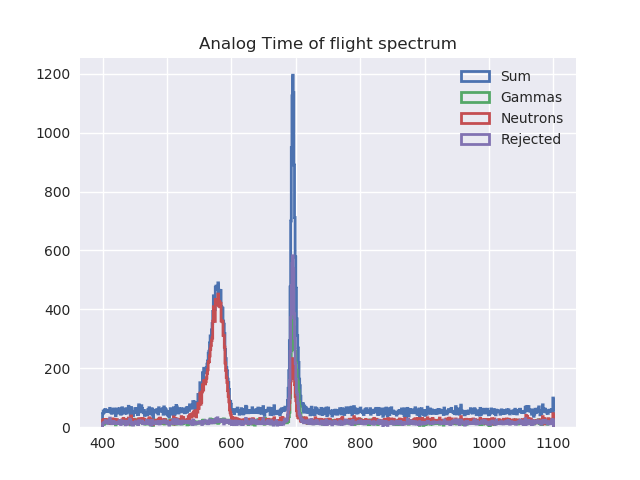
\includegraphics{AnalogResults/tof_psd.pdf}
        \caption{Time of flight plotted against PS. The dashed white line indicates the discrimination cut at tail/total = 0.259. A logarithmic z-axis is used to highlight the distribution of background events. Pedestal events have been removed with a cut at 0.8 $\text{MeV}_\text{ee}$.}
    \label{fig:tof_ps_a} 
\end{figure}

We can gain some more information on the effect of the injected pedestal events by looking at figure \ref{fig:tof_E_a}. Above 0.8 $\text{MeV}_\text{ee}$ We have a gamma and a neutron distribution as marked by the arrows. It is also clear that the events produced by triggering on YAP signals (less than 0.8 MeV) mostly land near the gamma ray time of flight. This is to be expected since these signals are acting as both start and stop signals. It is also clear that the cut at 0.8 $\text{MeV}_\text{ee}$ will not be able to remove all of these events. Unlike the gamma flash the neutron distribution show some correlation between time of flight and energy deposition. It seems that the faster neutrons are able to deposit more energy than the slower ones.

In figure \ref{fig:tof_Edep_Eneutron_a} the deposited energy is shown as a function of neutron kinetic energy as found from the time of flight spectrum. It can be seen that high energy deposition implies high neutron energy. However, the converse is not necessarily true as neutrons may scatter out of the detector before depositing all their energy. It is interesting that the energy the detector sees in $\text{MeV}_\text{ee}$ appears to be only half of the neutrons kinetic energy in  $MeV$.

\begin{figure}[ht]
    \centering
        \includegraphics{AnalogResults/tof_E.pdf}
        \caption{Time of flight plotted against energy deposition.}
    \label{fig:tof_E_a} 
\end{figure}

\begin{figure}[ht]
    \centering
        \includegraphics{AnalogResults/tof_Edep_Eneutron.pdf}
        \caption{Neutron energy as a function of deposited energy in the NE213 detector.}
    \label{fig:tof_Edep_Eneutron_a} 
\end{figure}




\end{document}
